%%%%%%%%%%%%%%%%%%%%%%%%%%%%%%%%%%%%%%%%%%%%%%%%%%%
%% Modèle de rapport pédagogique, doublé d'un tutoriel LaTeX
%% Vincent Labatut 2014-22 <vincent.labatut@univ-avignon.fr>
%%%%%%%%%%%%%%%%%%%%%%%%%%%%%%%%%%%%%%%%%%%%%%%%%%%
%% Classe du document
%\documentclass{ceri/sty/rapport}
% \documentclass[handout]{ceri/sty/rapport}
% \documentclass[light]{ceri/sty/rapport}
% \documentclass[full]{ceri/sty/rapport}
\documentclass[blue]{ceri/sty/rapport}
\usepackage{supertabular}



%%%%%%%%%%%%%%%%%%%%%%%%%%%%%%%%%%%%%%%%%%%%%%%%%%%
%% Informations générales
%%%%%%%%%%%%%%%%%%%%%%%%%%%%%%%%%%%%%%%%%%%%%%%%%%%
%TODO Formation concernée : à compléter.
% Exemples : Licence d'Informatique, Master d'Informatique.
\major{2ème année ENSC}


%TODO UE concernée par le rapport (à modifier).
% exemple : Projet Algorithmique
\course{Signal}


%TODO Titre du document, à adapter.
\title{Rapport de projet Réalité Augmentée}
% \subtitle{Sous-titre du document} % seulement si nécessaire

%TODO Liste des auteurs
\author{
	Dupont Clara \\ % il faut aller à la ligne entre chaque auteur
	Maigrot Jeanne \\
	Meunier Juliette \\
	Perret Quentin \\
    Tavard Hugo
}

%TODO Liste des encadrants, responsables d'UE, etc. (optionnel)
\advisor[Responsable]{ % indiquez ici le rôle (par défaut : "Encadrement")
	Marc Donias
}

%TODO Groupe des auteurs
% Optionnel : seulement si le travail est réalisé en groupe (en l'absence de groupe, ne définissez pas la macro)
% Exemple : Groupe 1, G12, etc.
\group{Groupe 2}

% Date de finalisation du rapport. 
% La valeur par défaut, qui est recommandée, est la date du jour.
\date{\today}
%\dateUpdt{}


%%%%%%%%%%%%%%%%%%%%%%%%%%%%%%%%%%%%%%%%%%%%%%%%%%%
%% Bibliographie
%%%%%%%%%%%%%%%%%%%%%%%%%%%%%%%%%%%%%%%%%%%%%%%%%%%
% Désigne le fichier bibliographique à utiliser
\addbibresource{bibliographie.bib}


%%%%%%%%%%%%%%%%%%%%%%%%%%%%%%%%%%%%%%%%%%%%%%%%%%%
%% Début du document
%%%%%%%%%%%%%%%%%%%%%%%%%%%%%%%%%%%%%%%%%%%%%%%%%%%
\setlength {\marginparwidth }{2cm}
\begin{document} 

% Création de la page de titre.
\maketitle

% Justification moins stricte : empêche certains mots de dépasser dans la marge
\sloppy      


%%%%%%%%%%%%%%%%%%%%%%%%%%%%%%%%%%%%%%%%%%%%%%%%%%%
%% Introduction
%%%%%%%%%%%%%%%%%%%%%%%%%%%%%%%%%%%%%%%%%%%%%%%%%%%
\section{Introduction}
\label{sec:Introduction}

Le remplacement de contenu sur vidéo, ainsi que sa détection est un procédé utilisé dans de nombreux domaines tels que le cinéma, la sécurité ou bien la photo pour citer quelques exemples. 
Dans le cadre de notre projet de réalité augmentée, le but était de réaliser un remplacement de contenu d’image ainsi que l’ajout d’une structure 3D. La vidéo originale présentait une feuille A4 bleue claire, sur laquelle était posé deux formes de Lego carrées. Cette feuille est au cours de la vidéo déplacée par une main présente sur le côté droit de la feuille. \\
\\
Ce projet fait place à plusieurs contraintes. Premièrement, tout le projet est à réaliser avec le langage de programmation Matlab et seules les fonctions basiques présentes dans le logiciel sont autorisées. Deuxièmement, lors de l’incrustation de l’image, il faut faire attention à ne pas recouvrir la main. Enfin, la structure 3D présente au-dessus de l’image doit se mouvoir en adéquation avec le déplacement de la feuille.\\
\\
Le travail a été séparé en trois parties. Tout d’abord, un binôme travaillait sur la détection des coins de la feuille. En parallèle, un trinôme était chargé de remplacer le contenu de la feuille par une nouvelle image 2D, en prenant en compte la main présente sur la vidéo. Enfin, nous nous sommes tous réunis pour travailler sur l’incrustation de contenu 3D.



%%%%%%%%%%%%%%%%%%%%%%%%%%%%%%%%%%%%%%%%%%%%%%%%%%%
%% Démarches théoriques
%%%%%%%%%%%%%%%%%%%%%%%%%%%%%%%%%%%%%%%%%%%%%%%%%%%
\section{Démarches théoriques}
\label{sec:Generalites1}



%%%%%%%%%%%%%%%%%%%%%%%%%%%%%%%%%%%%%%%%%%%%%%%%%%%
\subsection{Détection des coins}
\label{sec:OptionsClasse1}

 La détection et le suivi des points est le premier enjeu de ce projet. 
 Pour ce faire, nous avons commencé par calculer le gradient d'intensité en tout pixel, ce qui a permis de déterminer d'importantes variations d'intensité caractéristiques d'un fort contraste. \\
 Ainsi, les composantes horizontales et verticales du gradient ont été isolées à l'aide de l'approche de Canny (~\eqref{eq1}, ~\eqref{eq2}).
\begin{equation}
\label{eq1}
G_{x} ^{\sigma_G}(x,y)=  \frac{-x}{2\pi\sigma_G^4}e^\frac{x^2+y^2}{2\sigma_G^2}
\end{equation}
\begin{equation}
\label{eq2}
G_{y}^{\sigma_G}(x,y)=  \frac{-y}{2\pi\sigma_G^4}e^\frac{x^2+y^2}{2\sigma_G^2}
\end{equation}

Afin de détecter les coins, nous avons mis en place le filtre de Harris qui permet d'effectuer une analyse statistique du champ de gradient, et donc de l'exploiter. Pour sa réalisation, il a fallu calculer une  matrice de covariance qui met en évidence une organisation particulière de gradients, c'est à dire leurs auto-corrélations.

Pour calculer cette matrice, nous avons utilisé les dérivées en tout point, obtenues grâce aux résultats issus de l'approche de Canny précedemment effectuée : 
\begin{align}
\left\{
    \begin{array}{l}
        I_{x}^{\sigma_{G}} = I * G_{x}^{\sigma_{G}} \\
        I_{y}^{\sigma_{G}} = I * G_{y}^{\sigma_{G}}
    \end{array}
\right.
\end{align}

Ainsi, les différentes composantes de la matrice de covariances sont données par les formule suivantes : 
\begin{align}
\left\{
    \begin{array}{l}
        C_{xx}^{\sigma_G,\sigma_C} = (I_{x}^{\sigma_G}I_{x}^{\sigma_G})*G_{\sigma_{C}} \\
        C_{xy}^{\sigma_G,\sigma_C} = (I_{x}^{\sigma_G}I_{y}^{\sigma_G})*G_{\sigma_{C}} \\
        C_{yy}^{\sigma_G,\sigma_C} = (I_{y}^{\sigma_G}I_{y}^{\sigma_G})*G_{\sigma_{C}}
    \end{array}
\right.
\end{align}


Enfin, le déterminant de la matrice de covariance est calculé afin d'obtenir le détecteur de Harris en tout point : 

\begin{equation}
   D(x,y)= Det(C(x,y)) - \lambda Trace(C(x,y))^2
\end{equation}
 \\
 Le détecteur de Harris permet d'avoir des informations sur l'image en fonction de son signe : ses valeurs sont faibles si une région est d'intensité quasi constante, négatives au voisinage d'un contour et positives aux alentours d'un coin ce qui nous amène donc à la recherche d'un maximum, là où le coin se trouve.
\\
 
Dans l'objectif d'avoir une meilleur précision, nous avons calculé un autre détecteur de Harris, issu d'un changement dans la valeur du paramètre sigma. Ce dernier est comparé à l'ancien permettant d'obtenir un détecteur multi-échelle.
Cette combinaison multi-échelle est obtenue par la formule suivante : 

 \begin{equation}
   D = min(D_1^{\sigma_{G},\sigma_{C1}}|D_2^{\sigma_{G},\sigma_{C2}}|,|D_1^{\sigma_{G},\sigma_{C1}}|D_2^{\sigma_{G},\sigma_{C2}})
\end{equation}
\\
Afin d'améliorer le suivi de coins, nous avons utilisé le fait que les images sur lesquelles nous travaillions sont issues d'une vidéo, c'est à dire que les images ont un comportement dynamique et qu'elles dépendent les unes des autres. Ainsi, ces images ont des liens entre elles. Grâce à une trajectographie linéaire, il est possible de prédire la position des coins à l'avance en fonction de la détection des coins précédents. Pour ce faire, nous avons défini une fenêtre limitée à 37x37 pixels, réduisant la plage où la recherche d'un maximum dans le détecteur Harris s'effectue. 

\begin{figure}[H]
\centering
\includegraphics[scale=0.5]{images/Fenetre_Coin.PNG}
\caption{Fenêtre de détection de coin}
\end{figure}

 

%%%%%%%%%%%%%%%%%%%%%%%%%%%%%%%%%%%%%%%%%%%%%%%%%%%
\subsection{Remplacement de l'image}
\label{sec:OptionsClasse2}

\subsubsection{Réalisation de l'homographie}

Les coins de la feuille obtenus ont ensuite servi à calculer la matrice homographique permettant de projeter une image choisie sur la feuille de la vidéo. Cette matrice permet, à partir d'un vecteur contenant les positions initiales des pixels composant l'image à projeter, d'obtenir les nouvelles positions des pixels de cette image dans la vidéo, que l'on fixe avec à la position des coins. 

Afin d'obtenir cette matrice, nous avons dans un premier temps déterminé les coordonnées d'entrées de la matrice A grâce au système suivant :
\[
H = \begin{pmatrix}H_{11}&H_{12}&H_{13}\\
H_{21}&H_{22}&H_{23}\\
H_{31}&H_{32}&H_{33}
\end{pmatrix}  
\longleftrightarrow
\left \{ 
\begin{array}{cc}
 x_2= \frac{H_{11}x_1 + H_{12}y_1 + H_{13}}{H_{31}x_1 + H_{32}y_1 + H_{33}}  \\
 y_2= \frac{H_{21}x_1 + H_{22}y_1 + H_{23}}{H_{31}x_1 + H_{32}y_1 + H_{33}}  \\
\end{array}
\right .  
\]

Ce système permet d'obtenir la matrice A suivante, en notant ($x_2(i),y2(i)$) les coordonnées au point i de l'image à placer et ($x_1(i),y_1(i)$) les coordonnées correspondantes de la matrice homographique : \\
\\

$A = \begin{pmatrix}x_2(1)&y_2(1)&1&0&0&0&-x_2(1)*x_1(1)&-x_1(1)*x_2(1)\\ 
0&0&0&x_2(1)&y_2(1)&1&-x_2(1)*y_1(1)&-y_2(1)*y_1(1)\\ 
x_2(2)&y_2(2)&1&0&0&0&-x_2(2)*x_1(2)&-x_1(2)*x_2(2)\\ 
0&0&0&x_2(2)&y_2(2)&1&-x_2(2)*y_1(2)&-y_2(2)*y_1(2)\\ 
x_2(3)&y_2(3)&1&0&0&0&-x_2(3)*x_1(3)&-x_1(3)*x_2(3)\\ 
0&0&0&x_2(3)&y_2(3)&1&-x_2(3)*y_1(3)&-y_2(3)*y_1(3)\\ 
x_2(4)&y_2(4)&1&0&0&0&-x_2(4)*x_1(4)&-x_1(4)*x_2(4)\\ 
0&0&0&x_2(4)&y_2(4)&1&-x_2(4)*y_1(4)&-y_2(4)*y_1(4)\\ 
\end{pmatrix} $
\vspace{0.5cm}

Les coefficients de la matrice homographique X sont ensuite déterminés à l'aide de la relation suivante : 

 \begin{equation}
   A\times X=B \Leftrightarrow X=A^{-1}\times B
\end{equation}

Avec la matrice colonne B de taille $2i\times1$ représentant les coordonnées (x,y) des $i$ points de la feuille. Ici, $i=4$.
Ce calcul permet d'obtenir les coefficients de la matrice homographique mais sous un vecteur colonne. La matrice H est alors construite à partir de ces coefficients de manière à être de dimension 3x3 : \\
\\

$H = \begin{pmatrix}X(1)&X(2)&X(3)\\ 
X(4)&X(5)&X(6)\\ 
X(7)&X(8)&1\\ 
\end{pmatrix}$ 
\vspace{0.5cm}

Une fois cette matrice obtenue, l'homographie peut être réalisée en calculant le produit de convolution entre cette dernière et les coordonnées d'entrées. Afin de réaliser ce calcul, les coordonnées d'entrées doivent être homogènes d'où l'ajout d'un facteur d'échelle de 1. 
Une fois l'homographie réalisée, les coordonnées obtenues sont homogènes à un nouveau facteur d'échelle résultant des calculs réalisés. Ainsi, pour obtenir les coordonnées de l'image à remplacer il faut diviser le résultat de cette homographie par ce nouveau facteur d'échelle. 

\subsubsection{Détection de la main}
Une fois la matrice d'homographie calculée, il faut également prendre en compte la main présente au-dessus de la feuille pour que l'image que l'on ajoute ne la recouvre pas. 
La couleur de la main étant distinguable de celle de la feuille, nous avons choisi d'utiliser la méthode de segmentation colorimétrique afin d'isoler les pixels de la main. Cette segmentation s'est faite dans l'espace colorimétrique YCbCr.
Premièrement, les composantes RGB de l'image sont récupérées afin de calculer la luminance à l'aide de la formule suivante : 

\begin{equation}
   Y= 0.299*R+0.587*G+0.114*B
\end{equation}

Deuxièmement, pour se placer dans l'espace de chrominance rouge, permettant un meilleur contraste entre la feuille et la main, chaque pixel de l'image est transformé à l'aide de la formule suivante : 

\begin{equation}
   Cr=0.713*(R-Y)+128
\end{equation}
%
Enfin, les pixels sont discriminés par seuillage sous la condition Cr>129, valeur permettant d'isoler les pixels de la main tout en conservant ceux de la feuille. 

Une fois les pixels de la feuille récupérés, exceptés ceux de la main, l'homographie est réalisée et permet le remplacement de la feuille par notre image 

\begin{figure}[htb!]
\centering
\includegraphics [scale=0.3]{images/remplacement_pingu.png}
\caption{Remplacement de la feuille}
\label{fig:uapv}
\end{figure}

%%%%%%%%%%%%%%%%%%%%%%%%%%%%%%%%%%%%%%%%%%%%%%%%%%%
\subsection{Ajout d'un élement 3D}
\label{sec:OptionsClasse3}
Afin d'implémenter un élément 3D, il faut tout d'abord le créer. Nous avions depuis le début le désir de se concentrer sur un monde de glace. Après réflexion, nous avons décidé de créer un igloo. Ce dernier modélisé par une demie sphère que l'on construit grâce aux coordonnées sphériques : 
\\
\[
\left \{
   \begin{array}{l l l}
     x=\rho\times sin(\theta) \times cos(\alpha) \\
     y=\rho \times sin(\theta) \times sin(\alpha)  \\
     z=\rho \times cos(\alpha) 
    \end{array}
\right .
\]
Avec $\rho$ est le rayon que l'on décide de donner à l'igloo, $\theta = \frac{n_i}{2\rho}\times 2\pi$ et $\alpha = \frac{n_j}{2\rho}\times\frac{\pi}{2}$. L'objectif est donc d'avoir les matrices x,y,z carrées de tailles $2\rho\times2\rho$ représentant les coordonnées des points composants l'igloo. 
Pour être sûrs de la validité du modèle, nous avons tracé à l'aide de la fonction $plot3$ la demie-sphère. Une fois le modèle réalisé, il faut pouvoir passer de la 3D à la 2D. Pour ce faire, une matrice de projection $3D\longrightarrow2D$ fut construite dont le concept est similaire à l'homographie expliquée plus tôt, avec cette fois ci une quatrième colonne. Afin d'obtenir cette nouvelle matrice de projection, nous avons dans un premier temps déterminer les coordonnées d'entrées de la matrice A grâce au système suivant :
\vspace{0.5cm}
\[
P = \begin{pmatrix}P_{11}&P_{12}&P_{13}&P_{14}\\
P_{21}&P_{22}&P_{23}&P_{24}\\
P_{31}&P_{32}&P_{33}&P_{34}
\end{pmatrix}  
\longleftrightarrow
\left \{ 
\begin{array}{cc}
 x_2= \frac{P_{11}x_1^{3D} + P_{12}y_1^{3D} + P_{13}z_1^{3D} + P_{14}}{P_{31}x_1^{3D} + P_{32}y_1^{3D} + P_{33}z_1^{3D} + P_{34}}  \\
 y_2= \frac{P_{21}x_1^{3D} + P_{22}y_1^{3D} + P_{23}z_1^{3D} + P_{24}}{P_{31}x_1^{3D} + P_{32}y_1^{3D} + P_{23}z_1^{3D} + P_{34}}  \\
\end{array}
\right .  
\]
\vspace{0.5cm}
Ce système permet d'obtenir la matrice A suivante, en notant ($x_2(i),y_2(i),z_2(i)$) les coordonnées au point i de l'image à placer et ($x_1(i),y_1(i),z_1(i)$) les coordonnées correspondantes de la matrice homographique : \\
\\
\vspace{0.5cm}
\hspace{-0.5cm}
\setcounter{MaxMatrixCols}{11}
$A = \begin{pmatrix}x_2(1)&y_2(1)&z_2(1)&1&0&0&0&0&-x2(1)*x1(1)&-x1(1)*x2(1)&-x_2(1)*z_2(1)\\ 
0&0&0&0&x2(1)&y2(1)&z_2(1)&1&-x_2(1)*y_1(1)&-y_2(1)*y_1(1)&-y_2(1)*z_2(1)\\ 
x_2(2)&y2(2)&z_2(2)&1&0&0&0&0&-x_2(2)*x_1(2)&-x_1(2)*x_2(2)&-x_2(2)*z_2(2)\\ 
0&0&0&0&x2(2)&y2(2)&z_2(2)&1&-x_2(2)*y_1(2)&-y_2(2)*y_1(2)&-y_2(2)*z_2(2)\\ 
x_2(3)&y2(3)&z_2(3)&1&0&0&0&0&-x_2(3)*x_1(3)&-x_1(3)*x_2(3)&-x_2(3)*z_2(3)\\ 
0&0&0&0&x2(3)&y2(3)&z_2(3)&1&-x_2(3)*y_1(3)&-y_2(3)*y_1(3)&-y_2(3)*z_2(3)\\ 
x_2(4)&y2(4)&z_2(4)&1&0&0&0&0&-x_2(4)*x_1(4)&-x_1(4)*x_2(4)&-x_2(4)*z_2(4)\\ 
0&0&0&0&x2(4)&y2(4)&z_2(4)&1&-x_2(4)*y_1(4)&-y_2(4)*y_1(4)&-y_2(4)*z_2(4)\\ 
x_2(5)&y2(5)&z_2(5)&1&0&0&0&0&-x_2(5)*x_1(5)&-x_1(5)*x_2(4)&-x_2(5)*z_2(5)\\ 
0&0&0&0&x2(5)&y2(5)&z_2(5)&1&-x_2(5)*y_1(5)&-y_2(5)*y_1(5)&-y_2(5)*z_2(5)\\ 
\end{pmatrix} $
\vspace{0.5cm}

Les coefficients de la matrice de projection P sont ensuite déterminés à l'aide de la relation suivante : 
\\

 \begin{equation}
   A*P=B \Leftrightarrow P=A^{-1}*B
\end{equation}

Avec la matrice colonne B de taille $2i\times1$ représentant les coordonnées (x,y) des $i$ points de la feuilles. Ici, $i=5$.
Ce calcul permet d'obtenir les coefficients de la matrice de projection mais sous un vecteur colonne. La matrice P est alors construite à partir de ces coefficients de manière à être de dimension 3x4 : \\
\\

$H = \begin{pmatrix}P(1)&P(2)&P(3)&P(4)\\ 
P(5)&P(6)&P(7)&P(8)\\ 
P(9)&P(10)&P(11)&1\\ 
\end{pmatrix}$ 
\vspace{0.5cm}

Une fois cette matrice obtenue, la projection peut être réalisée en calculant le produit de convolution entre cette dernière et les coordonnées d'entrées. Afin de réaliser ce calcul, les coordonnées d'entrées doivent être homogènes d'où l'ajout d'un facteur d'échelle de 1. 
Une fois la projection réalisée, les coordonnées x et y obtenues sont homogènes à un nouveau facteur d'échelle résultant des calculs réalisés. Ainsi, pour obtenir les coordonnées de l'image à remplacer il faut diviser le résultat de cette projection par ce nouveau facteur d'échelle.

%%%%%%%%%%%%%%%%%%%%%%%%%%%%%%%%%%%%%%%%%%%%%%%%%%%
%% Réalisation
%%%%%%%%%%%%%%%%%%%%%%%%%%%%%%%%%%%%%%%%%%%%%%%%%%%
\section{Réalisation}
\label{sec:Réalsiation}

\subsection{Architecture}

Ci-dessous, il est présenté notre architecture de code avec le différentes fonctions et leurs liens entre elles.

\begin{figure}[H]
\centering
\includegraphics[width=\textwidth]{images/diagramme.png}
\caption{Architecture des fonctions présentes dans notre code} %revoir nom
\end{figure}


\subsection{Fonctions}
\label{sec:OptionsClasse4}

\begin{table}[H]
\caption{Table des fonctions crées}
\centering
\rowcolors{1}{fgVeryLightRed}{}
\begin{tabular}{m{3.5cm} m{3cm} m{1.5cm} m{6cm}}
\hline
\rowcolor{fgLightRed}
\textbf{Nom Fonction} & \textbf{Entrée} & \textbf{Sortie} & \textbf{Description} \\
\hline
CouleurToGris& Image & & Permet de passer une image en vraies couleurs en couleurs indexées \\
Canny & Image, sigma & $I_x$, $I_y$ & Estime les dérivées en tout point selon x et y \\
Harris & sigma, sigmaG, image & detecteur & Calcul du détecteur de Harris combinant trace et déterminant\\ 
HarrisMultiEchelle& sigma1, sigma2, sigmaG, image & detecteurMulti& Détermine le meilleur détecteur de Harris pour 2 valeurs de sigma \\
ValMaxHarris & detecteur, posEncoreAvant,posAvant & posMax & Recherche de la valeur maximale du detecteur de Harris dans une fenêtre donnée \\
DetectCoin & detecteur, coinsImage1,coinsImage2 & coins & Détermine les coordonnées des coins de la feuille\\
Homographie & x1,y1,x2,y2, nbpts & H & Calcule la matrice homographique à partir des coins de la feuille \\
DetectMain & frame & M & Récupère les coordonnées de la feuille isolées de celles de la main à l'aide d'un seuillage dans le modèle YCbCr\\
Replace & frame,img,H & frame & Remplace les pixels de la feuille par ceux de l'image à ajouter tout en conservant ceux de la main\\
Igloo & diametre,numeroFrame & x,y,z & Créer un igloo et renvoie les coordonnées 3D\\
RecuperePoints & x,y,z, taille & pointsARelier & Renvoie les points à relier afin de tracer l'igloo\\
Projection3D & x1,y1,P3D,nbpts & P & Calcule la matrice de projection permettant de passer des coordonnées 3D aux coordonnées 2D\\
Trace & frame, pts3D & frame & Trace l'igloo sur la frame de la vidéo\\
RemplaceVerif3D & frame, pointsARelier, P & frame & Ajoute la structure 3D à la frame de la vidéo 
%vérifier s'il manque des fonctions
\end{tabular}
\label{tab:exemple1}
\end{table}

\begin{table}[H]
\caption{Table des fonctions Matlab utilisées}
\centering
\rowcolors{1}{fgVeryLightRed}{}
\begin{tabular}{m{4cm} m{2cm} m{2cm} m{6cm}}
\hline
\rowcolor{fgLightRed}
\textbf{Nom Fonction} & \textbf{Entrée} & \textbf{Sortie} & \textbf{Description} \\
\hline

VideoReader & filename & v &  Permet de lire un fichier vidéo\\
VideoWriter & filename & v & Créer un objet capable de créer une vidéo à partir d'une matrice\\
imread & filename & M & Retourne l'image d'entrée sous forme d'un tableau \\
read & filename & frame & Permet de lire une ou plusieurs frame de la vidéo\\
writeVideo & v (vidéo), img & frame & Créer une ou plusieurs frame sur une vidéo\\
getframe & gfc & frame & Récupère la frame d'une vidéo \\
conv2& X,Y & Z & Retourne la convolution 2D des matrices A et B\\
max & x,y & z & Renvoie le maximum entre x et y \\
min & x,y & z & Renvoie le minimum entre x et y\\
abs & x & z & Renvoie la valeur absolue du nombre x\\
double & X & Y & Convertit chaque élément de X en un double\\
round & X & X' & Arrondit chaque élément de la matrice à l'entier le plus proche \\
ceil& a & b & Arrondit l'entier à l'arrondi le plus proche, dans le sens des positifs \\
size & X & [x y] & Renvoie la taille de la matrice selon chaque dimension\\
length & X & n & Renvoie la longueur de la plus grande dimension de X\\
zeros & i,j & M & Créer une matrice de 0 de dimension $ixj$ \\
meshgrid & x,y & X,Y & Renvoie des coordonnées d'une grille 2D basées sur les coordonnées des vecteurs x et y. X est une matrice où chaque ligne est une copie de x, et Y est une matrice où chaque colonne est une copie de y. La grille représentée par les coordonnées X et Y a longueur(y) lignes et longueur(x) colonnes.\\
plot & X,Y & & Créer un graphique où sont tracés X et Y\\
%vérifier s'il manque des fonctions
\hline
\end{tabular}
\label{tab:exemple2}
\end{table}


%%%%%%%%%%%%%%%%%%%%%%%%%%%%%%%%%%%%%%%%%%%%%%%%%%%
\subsection{Variables}
\label{sec:OptionsClasse5}


\begin{table}[H]
\caption{Table des variables utilisées}
\centering
\rowcolors{1}{fgVeryLightRed}{}
\begin{tabular}{m{5cm} m{4cm} m{6cm}}
\hline
\rowcolor{fgLightRed}
\textbf{Nom Variable} & \textbf{Type} & \textbf{Description} \\
\hline

nbFrame & entier & Nombre de frames de la vidéo \\
sigma1, sigma2, sigmaG & entiers & Paramètres fonctionnels du détecteur de Harris multi-échelle \\
coinsPreviousFrame & Matrice de doubles & Coordonnées des points de la feuille détectés sur l'image précédente (ici les 4 coins + 2 points) \\
coinsFrame & Matrice de doubles & Coordonnées des points de la feuille détectés sur l'image actuelle \\
meme & Matrice d'entiers & Image à incruster, sous forme de matrice de pixels \\
taille & Matrice d'entiers & Taille de l'image à incruster \\
x2, y2 & Vecteurs d'entiers & Coordonnées 2D des 4 coins de l'image à incruster \\
P3D & Matrice de doubles & Coordonnées 3D des 4 coins de l'image à incruster \\
img & Matrice de doubles & Une image de la vidéo qui va être traitée et remplacée \\
HarrisFinal & Matrice de doubles & Valeur du détecteur de Harris final \\
x1, y1 & Vecteurs d'entiers & Coordonnées 2D des points de la feuille détectés \\
X & Matrice de doubles & Matrice Homographique \\
newim & Matrice de doubles & Nouvelle image après insertion de l'image à incruster dans l'image de la vidéo  \\
x, y, z & Matrices de doubles & Coordonnées 3D des points formant l'igloo \\
pointsARelier & Matrice de doubles & Coordonnées 3D des points de l'igloo, ordonnés de façon à pouvoir les relier simplement \\
P & Matrice de doubles & Matrice de Projection 3D vers 2D \\
im & Matrice de doubles & Image finale de la vidéo avec l'image incrustée et la structure 3D \\



%vérifier s'il manque des fonctions
\hline
\end{tabular}
\label{tab:exemple3}
\end{table}



%%%%%%%%%%%%%%%%%%%%%%%%%%%%%%%%%%%%%%%%%%%%%%%%%%%
%% Résultats
%%%%%%%%%%%%%%%%%%%%%%%%%%%%%%%%%%%%%%%%%%%%%%%%%%%
\section{Résultats}
\label{sec:Generalites3}

\subsection{Détection des coins}

Afin de vérifier que nous allions sur la bonne voie, nous avons vérifié nos résultats au fur et à mesure, notamment, avec le détecteur de Harris. Avant d'aller plus loin, nous avons affiché les différents détecteurs, ainsi que le détecteur multi-échelle (figure \ref{fig:subfigures2}). Nous pouvons voir les 4 coins de la feuille, de même que les structures 3D comme nous le souhaitions.

\begin{figure}[H]
\centering
\begin{subfigure}[t]{0.3\textwidth}
\includegraphics[width=\textwidth]{images/harris1.PNG}
\caption{Détecteur de Harris pour \sigma=2}
\label{fig:subfig2}
\end{subfigure}
\hfill
\begin{subfigure}[t]{0.3\textwidth}
\includegraphics[width=\textwidth]{images/harris2.PNG}
\caption{Détecteur de Harris pour \sigma=5}
\end{subfigure}
\hfill
\begin{subfigure}[t]{0.3\textwidth}
\includegraphics[width=\textwidth]{images/harris3.PNG}
\caption{Détecteur de Harris MultiEchelle}
\end{subfigure}
\caption{Détecteurs de Harris}
\label{fig:subfigures2}
\end{figure}



Nous avons ensuite vérifié si suite à la prédiction linéaire, les coins étaient bien reconnus tout au long de la vidéo. Comme l'on peut le voir sur la figure\ref{fig:coin1}, les quatre coins sont bien reconnus. 


\begin{figure}[H]
\centering
\includegraphics[scale=0.3]{images/signal1.png}
\caption[coin1]{Capture d'écran d'une image de la vidéo avec les 4 coins détectés}
\label{fig:coin1}
\end{figure}


Pour ajouter de la stabilité pour l'homographie, nous avons rajouté un point au centre de la feuille, comme l'on peut le voir sur la figure \ref{fig:coin2}.

\begin{figure}[H]
\centering
\includegraphics[scale=0.4]{images/signal2.png}
\caption[coin2]{Capture d'écran d'une image de la vidéo avec les 4 coins détectés et un point central}
\label{fig:coin2}
\end{figure}

Des améliorations sont possible pour la détection de coin, notamment en se concentrant sur le seuil ou bien la fenêtre de repérage du maximum dans le détecteur de Harris.

\subsection{Homographie}
% test sur une frame, en indiquant les coins à la main (ginput)
% idem ensuite avec ajout de la gestion de la main
% --> en vrai bon résultat donc on a gardé comme ça
% ensuite quand on a eu la partie détections des points on a vu que c'etait pas hyper stable avec seulement nos 4 coins
% --> ajout de deux autres points pour plus de stabilité

Afin de s'assurer du bon fonctionnement de notre fonction homographique nous l'avons testée à de nombreuses reprises, en indiquant les coins de la feuille "à la main" puisque la partie "détection des coins" n'était pas encore achevée. Nous avons pour cela utilisé la fonction \textit{ginput} de Matlab. En appliquant notre homographie à la première frame de la vidéo nous avons pu observer un résultat satisfaisant (cf figure \ref{fig:homographie1}).

\begin{figure}[H]
\centering
\includegraphics[scale=0.3]{images/homographie1.png}
\caption[homographie1]{Capture d'écran de la première frame de la vidéo avec l'image ajoutée à partir de 4 points}
\label{fig:homographie1}
\end{figure}

Après ajout de la gestion de la main (par seuillage dans un espace colorimétrique YCbCr), nous avons testé de nouveau notre homographie mais cette fois sur une frame plus tardive afin d'avoir la main sur la feuille. Nous avons alors pu voir que notre fonction était tout à fait convenable (cf figure \ref{fig:homographie2}) et nous n'avons pas jugé nécessaire de faire une approche elliptique pour la détection de la main, bien que cette dernière soit jugée plus efficace de manière générale.

\begin{figure}[H]
\centering
\includegraphics[scale=0.3]{images/homographie2.png}
\caption[homographie2]{Capture d'écran de la quarantième frame de la vidéo avec l'image ajoutée}
\label{fig:homographie2}
\end{figure}

Enfin, lorsque nous avons eu la fonction de détection des coins, nous avons pu tester notre fonction homographique sur l'ensemble de la vidéo. Nous avons alors remarqué une certaine instabilité de l'image lors du déplacement de la feuille. C'est pourquoi nous avons décidé d'ajouter un autre point, situé au centre de l'image. La stabilité de l'image a alors été grandement augmentée.

\begin{figure}[H]
\centering
\includegraphics[scale=0.3]{images/homographie3.png}
\caption[homographie3]{Capture d'écran de la quarantième frame de la vidéo avec l'image ajoutée à partir de 5 points}
\label{fig:homographie2}
\end{figure}



\subsection{Élément 3D}

A l'aide du modèle de l'igloo et de la fonction $Projection3D$ nous pouvons désormais obtenir les coordonnées $2D$ des points de la demie-sphère. La fonction $Replace3D$, de concert avec la fonction $Trace$ permettent de tracer sur les images de la vidéo l'igloo. 
Cependant, une difficulté subsiste, comment savoir quel point relier avec quel point pour en tracer le segment ? 
Pour y répondre, nous avons du nous renseigner sur l'indexation par défaut que $Matlab$ effectue sur ses matrices. Avec ces informations, nous savons désormais que chaque point doit être relié à celui du dessous mais aussi à celui de la colonne de droite (quant à la dernière colonne, elle doit être reliée à la première pour fermer la demie sphère). Ainsi, en sortie de la fonction $Igloo$, nous faisons appel à la fonction $RecuperePoints$ qui se charge de classer les points dans l'ordre dans une matrice de taille $Nombre de points \times 3$ (3 pour x,y,z), qui sera plus facile à traiter pour les fonctions graphiques. La position de l'igloo a été choisie arbitrairement. Les images ainsi obtenues sont les suivantes : 

\begin{figure}[H]
\centering
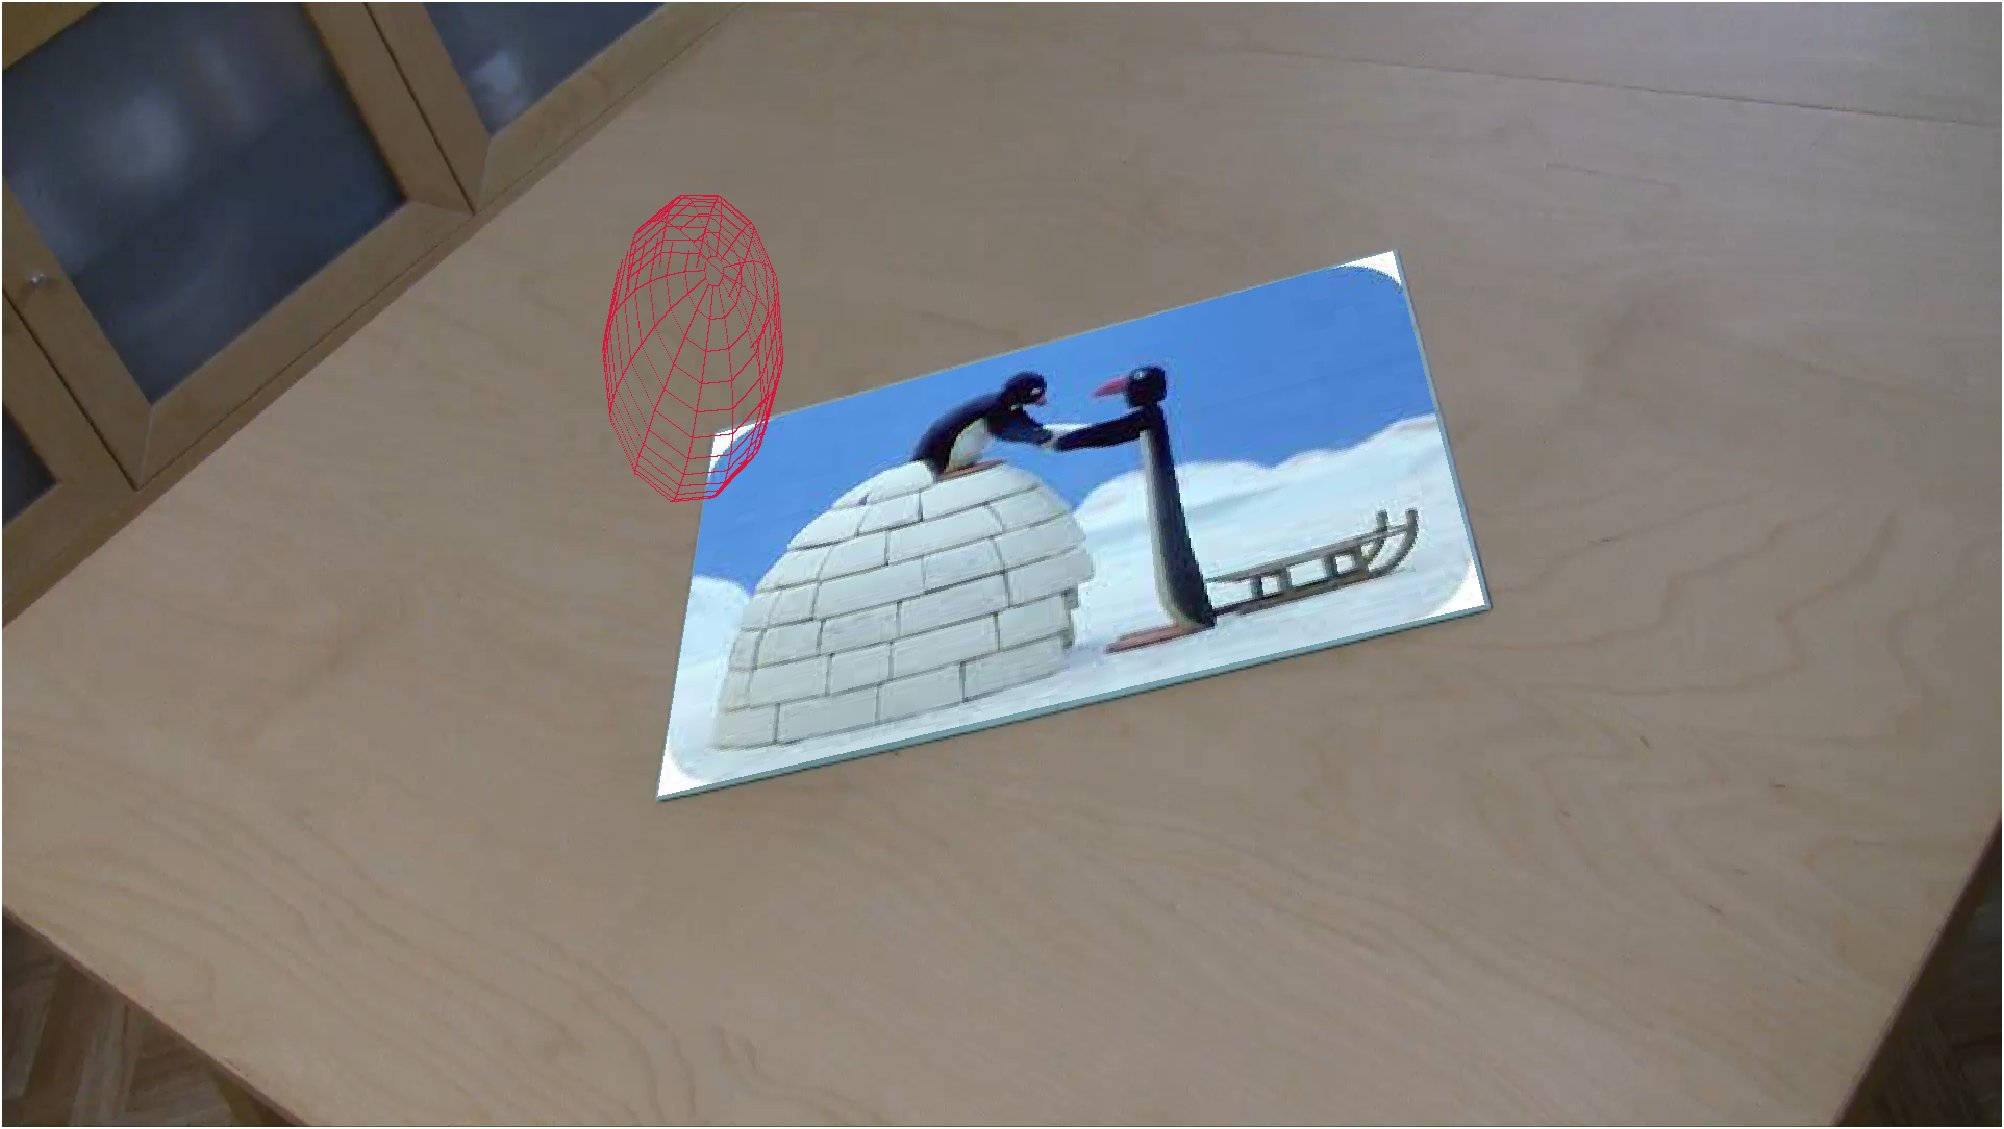
\includegraphics[scale=0.3]{images/proj3D_1.png}
\caption[proj3D1]{Capture d'écran de la première frame de la vidéo avec l'image et l'élément 3D ajoutée}
\label{fig:uapv}
\end{figure}

\begin{figure}[H]
\centering
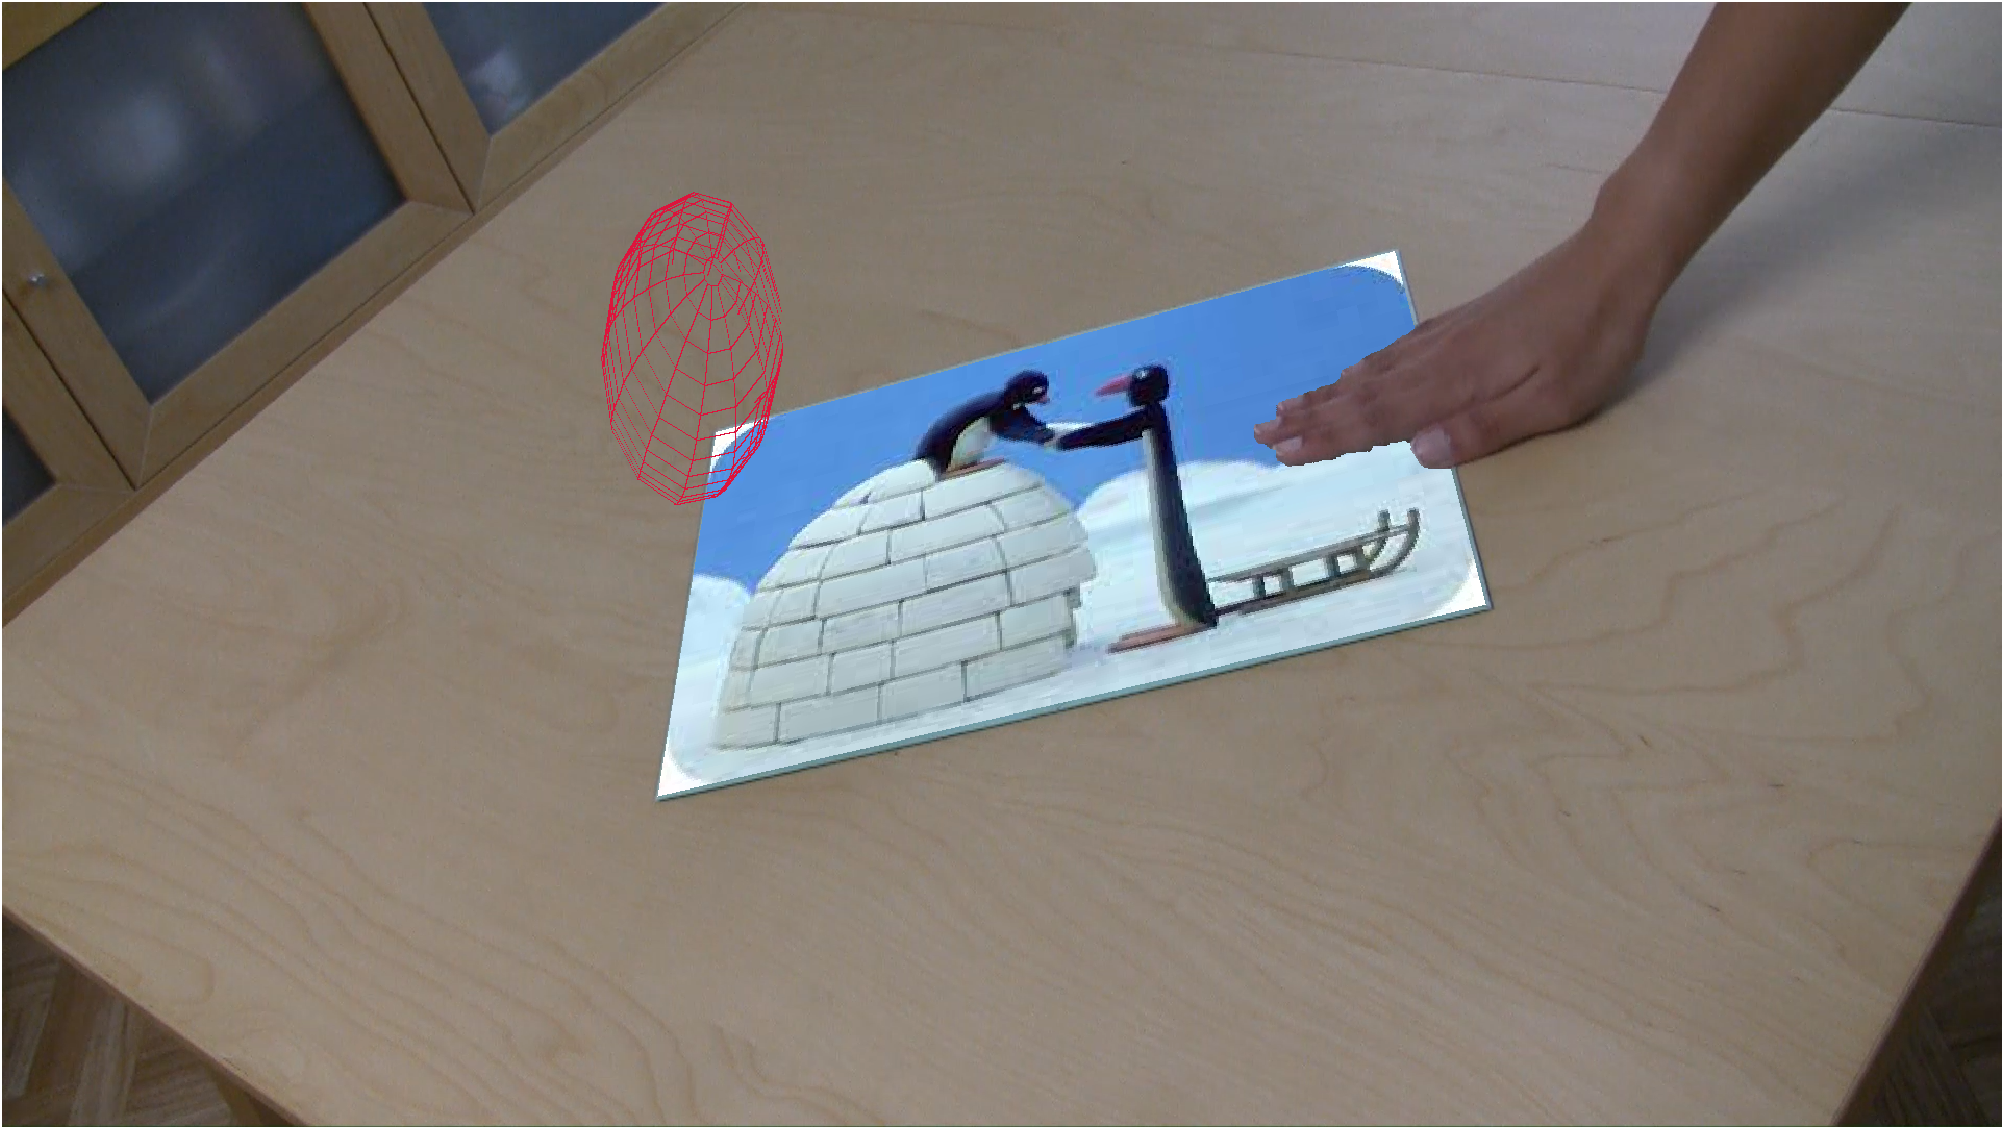
\includegraphics[scale=0.3]{images/proj3D_2.png}
\caption[proj3D2]{Capture d'écran de la quarantième frame de la vidéo avec l'image et l'élément 3D ajoutée}
\label{fig:uapv}
\end{figure}

Finalement le temps d'exécution total est de 305,10 secondes. 
%%%%%%%%%%%%%%%%%%%%%%%%%%%%%%%%%%%%%%%%%%%%%%%%%%%
%% Organisation
%%%%%%%%%%%%%%%%%%%%%%%%%%%%%%%%%%%%%%%%%%%%%%%%%%%
\section{Gestion de projet}
\label{sec:Generalites4}


\subsection{Répartition du travail et coordination}
Comme indiqué dès la première séance de travail,  nous nous sommes divisés en deux groupes. Un binôme composé de Hugo Tavard et Juliette Meunier, responsable de la détection des coins (en violet sur la figure 
 \ref{fig:uapv}). Et un deuxième trinôme composé de Clara Dupont, Jeanne Maigrot et Quentin Perret était chargé d'effectuer l'homographie afin de pouvoir remplacer l'image et identifier la main (en jaune sur la figure  \ref{fig:uapv}).
\\

Nous avons mis ensuite en commun nos deux codes afin de pouvoir commencer la troisième partie, l'ajout d'une figure 3D. Pour cette dernière partie, nous avons redivisé le travail en deux : il fallait commencer par rendre la détection des coins plus robuste mais aussi adapter la fonction homographie pour faire une fonction de projection 3D. Enfin, nous nous sommes réunis pour la dernière étape en vue de commencer d'une part le rapport et d'autre part, ajouter la figure 3D choisie, un igloo.
\\

Nous avons utilisé à notre avantage les plages de TD pour travailler où nous avons pu avancer par binôme ou trinôme, mais en se tenant au courant des progrès de l'autre équipe. Cependant, un large travail personnel fut nécessaire pour terminer ce projet à temps.  

\begin{figure}[H]
\centering
\includegraphics[scale=0.15]{images/Planning.png}
\caption[planning]{}
\label{fig:uapv}
\end{figure}

\subsection{Outils utilisés}
Comme le projet est à réaliser sur Matlab, nous avons bien entendu utilisé le langage Matlab. Pour pouvoir partager nos avancées et versionner notre code, nous avons placé Git à l'honneur.
Enfin, pour le rapport, nous avons utilisé \LaTeX  pour pouvoir écrire les équations mathématiques de manière plus facile, pratique et pour que leur police soit plus agréable à lire.
Enfin, afin de s'organiser, notamment en ce qui concerne la rédaction du rapport et la finalisation du code, nous avons communiqué par Messenger.


%%%%%%%%%%%%%%%%%%%%%%%%%%%%%%%%%%%%%%%%%%%%%%%%%%%
%% Conclusion
%%%%%%%%%%%%%%%%%%%%%%%%%%%%%%%%%%%%%%%%%%%%%%%%%%%
\section{Conclusion}
Ce projet a été l'occasion de mettre en pratique les approches théoriques vues lors des cours et de d'approfondir notre maîtrise du logiciel Matlab. Le fait de coder nous-même les fonctions nécessaires au remplacement d'une image nous plus particulièrement permis d'avoir une compréhension plus concrète et technique de ce dernier. De même en ce qui concerne le cours, certains points d'ombre ont pu être éclaircis de par les attentes du projet. 
Durant ce dernier, plusieurs difficultés ont pu être rencontrées pour la réalisation des différentes étapes que ce soit en termes d'approche ou de réalisation. Cependant, ces difficultés ont pu être surmontées et elles ne nous ont pas empêchées d'obtenir des résultats satisfaisants : les coins de l'image ont pu être détectés afin de pouvoir remplacer la feuille par une image sans écraser la main. Concernant l'ajout de contenu 3D, nous avons réussi à ajouter une structure d'igloo rotatif en 3D même si nous n'avons pas réussi à réaliser parfaitement ce que l'on souhaitait. Néanmoins, le code est fonctionnel, et le groupe reste satisfait du travail effectué.

%%%%%%%%%%%%%%%%%%%%%%%%%%%%%%%%%%%%%%%%%%%%%%%%%%%
%% Réalisation
%%%%%%%%%%%%%%%%%%%%%%%%%%%%%%%%%%%%%%%%%%%%%%%%%%%
\section{Annexe}
Notre code se trouve sur le dépôt GitHub suivant : 

\url{https://github.com/QuentinPerret/SignalProject.git}.

%%%%%%%%%%%%%%%%%%%%%%%%%%%%%%%%%%%%%%%%%%%%%%%%%%%
%% Bibliographie
%%%%%%%%%%%%%%%%%%%%%%%%%%%%%%%%%%%%%%%%%%%%%%%%%%%
\MyBibliography


\end{document}
